\documentclass[parskip=full]{scrartcl}

\usepackage[utf8]{inputenc} % use utf8 file encoding for TeX sources
\usepackage[T1]{fontenc} % avoid garbled Unicode text in pdf
\usepackage[german]{babel} % german hyphenation, quotes, etc
\usepackage{hyperref} % detailed hyperlink/pdf configuration
\usepackage{mathptmx} %Schriftart Times
\usepackage[scaled]{helvet} %
\usepackage{graphicx}
\hypersetup{ % ‘texdoc hyperref‘ for options
pdftitle={Pflichtenheft},
bookmarks=true,
}
\usepackage{csquotes} % provides \enquote{} macro for "quotes"
%TitlePage
{\title{\fontsize{40}{48} \selectfont \textsc{Pflichtenheft-Entwurf}\\
{\fontsize{18}{18} \selectfont Multimediatool zum Testen von Videoencodern}}}
{\author{Carina, Ben, Johannes, Noel, Sascha, Simon}}

\begin{document}
\maketitle
\thispagestyle{empty}
\newpage
\tableofcontents
\newpage
\section{Zielbestimmung}
Mit dem Produkt sollen Firmen/Forschungsprojekte eine einfache Möglichkeit erhalten,
verschiedene Videoencoder objektiv zu bewerten und mit einander zu vergleichen.
\subsection{Musskriterien}
\subsubsection{Encoder auswählen}
\begin{itemize}
\item Der Benutzer kann einen eigenen Encoder auswählen
\item Der Benutzer kann aus einer Liste kürzlich benutzter Encoder auswählen
\end{itemize}
\subsubsection{Video Auswählen}
\begin{itemize}
\item Der Benutzer kann ein Video zum encodieren auswählen
\item Der Benutzer kann aus einer Liste kürzlich encodeder Videos auswählen
\item Der Benutzer kann aus einer Liste von Filtern einen Filter auswählen und diesen auf
das gesamte Video anwenden
\item Der Benutzer kann aus einer Liste von Artefakten ein Artefakt auswählen und dieses
in das gesamte Video einfügen
\item Der Benutzer bekommt vor dem Anwenden der Artefakte oder Filter eine Vorschau angezeigt
\item Nach dem Anwenden der Filter und Artefakte hat der Nutzer die Chance das Video komplett
anzuschauen
\end{itemize}
\subsubsection{Codieren des Videos}
\begin{itemize}
\item Der Benutzer kann das ausgewählte und angepasste Video mit dem ausgewählten Encoder Codieren
\end{itemize}
\subsubsection{Bewerten des Encoders}
\begin{itemize}
\item Der Benutzer kann das Rohevideo und das encodierte Video synchron nebeneinander anschauen
\item Der Benutzer kann die im vorigen Punkt genannten Videos in einstellbarer Geschwindigkeit
Abspielen
\item Der Benutzer kann sich berechnete Bewertungskriterien für den Encoder anzeigen lassen
\item Der Benutzer kann sich Unterschiede zwischen Roh- und encodiertem Video anzeigen lassen
\item Der Benutzer kann sich interressante (encoderspezifische) Eigenschaftem im encodiertem
Video anzeigen lassen
\end{itemize}
\subsection{Wunschkriterien}
\begin{itemize}
\item Bewertungen in Datenbank speichern
\item Bewertungen aus Datenbank laden und neben der Bewertung des aktuell geladenen Encoders anzeigen
\end{itemize}
\subsection{Abgrenzungskriterien}
\begin{itemize}
\item Es wird keine Dokumentation mitgeliefert
\item Die Software ist ausschließlich in deutscher Sprache verfügbar
\item Die GUI ist fest vorgegeben, d.h. Schriftart,-größe, etc. sind nicht veränderbar
\end{itemize}
\section{Produkteinsatz}
Das Produkt dient zum Testen und Vergleichen von Videoencodern. 
Damit sollen sowohl Privatpersonen, als auch Firmen oder Forschungseinrichtungen darin unterstützt werden, den best möglichen Videoencoder für ihre Bedürfnisse zu finden.
\subsection{Anwendungsbereiche}
Vergleich von Videoencodern für verschiedene Bedürfnisse
\subsection{Zielgruppe}
\begin{itemize}
\item Anwender von Videoencodern/ Privatpersonen
\item Hersteller von Videoencodern
\item Videoediteure
\item Graphikdesigner
\item Cutter
\item Videoplattformbetreiber
\item Forschungseinrichtungen
\end{itemize}
\subsection{Betriebsbedingungen}
\begin{itemize}
\item Benutzbar rund um die Uhr
\item Wartungsfrei
\item In privat oder geschäftlichem Einsatz
\end{itemize}
\section{Produktumgebung}

\subsection{Hardware}
Für die Software wird ein 64 Bit Betriebssystem benötigt, welches einen 64 Bit Prozessor voraussetzt.

\subsection{Software}
\begin{itemize}
\item 64Bit Linux
\item Qt Bibliothek Version 5.6.0
\end{itemize}

\section{Funktionale Anforderungen}
\subsection{Encoder auswählen}
Der Benutzer kann mittels eines Dateiauswahldialogs eine ausführbare Datei (ELF32,ELF64) auswählen.
Das Programm muss ein über das Terminal gestartet werden können und das zu encodende Video als
Argument übernehmen.
Zudem hat der Benutzer die Möglichkeit, einen Encoder aus einer Liste zu wählen, in der die letzten 5 zuvor
verwendeten Encoder stehen. Das Programm prüft vor dem Anzeigen der Encoder ob diese noch existieren.
\subsection{Video auswählen}
Der Benutzer kann mittels eines Dateiauswahldialogs ein Video auszuwählen. Dieses
Video wird später encodiert. Der Benutzer hat die Möglichkeit ein Video aus einer Liste zu wählen, die die letzten 10 encodierten
Videos enthält. Das Programm prüft vor dem Anzeigen der Videos, ob diese noch existieren.
\subsection{Filter auswählen}
Der Benutzer hat die Möglichkeit einen einzigen Filter aus einer Liste vorgefertigter Filter mithilfe von Checkboxen auszuwählen. Vorhandene Filter:
\begin{itemize}
\item Schwarzweiß-Filter
\item Unschärfe-Filter
\item Farbfilter
\end{itemize}
\subsection{Artefakte auswählen}
Der Benutzer hat die Möglichkeit ein einziges Artefakt/Muster aus einer Liste vorgefertigter
Artefakte/Muster auszuwählen. Diese Liste enthält folgende:
\begin{itemize}
\item Gitter-Muster
\end{itemize}
\subsection{Vorschau anzeigen}
Der Benutzer hat die Möglichkeit, wenn er ein Artefakt oder ein Muster ausgewählt hat, sich eine
Vorschau anzeigen zu lassen. Diese Vorschau besteht aus 5 Frames. Diese Frames sind jeweils bei
1/5,2/5,... der gesamten Frameanzahl entnommen. Auf diese Frames wird der Filter bzw. Artefakt
angewendet. Der Benutzer kann durch alle 5 Frames durchschalten. Wurde ein Artefakt und ein Filter
gleichzeitig ausgewählt, wird erst das Artefakt angewendet, dann der Filter und wird die
Vorschau angezeigt.
\subsection{Filter/Artefakte anwenden}
Der Benutzer muss den Filter/Artefakt anwenden, bevor das Video damit encodiert wird. Tut er
das nicht, wird das Originalvideo codiert. Wenn der Nutzer das originale Video verändert, wird eine neue Videodatei mit
dem Filter/Artefakt erzeugt. Werden Filter oder Artefakte geändert und die Änderungen angewandt, wird wieder eine neue
Datei erstellt und die vorherige wieder gelöscht.
\subsection{Vorschau des kompletten Videos}
Hat der Benutzer den Filter/Artefakt angewandt, hat er die Möglichkeit, sich das komplette, neue
Video anzuschauen. Steuerelemente für das Video sind dabei lediglich ein Start, Pause und Restart Buttons.
\subsection{Video Encodieren}
Der Benutzer kann, wenn er ein Video und Encoder ausgewählt hat, das ausgewählte Video mit dem ausgewählten Encoder codieren.
\subsection{Bewertung des Encoders}
\subsubsection{Amschauem des codierten und rohen Videos}
Der Benutzer kann das Rohvideo sowie das codierte anschauen. Dabei sind beide Videos gleichzeitig zu sehen. Steuerelemente sind Start, Pause und Stop sowie eine Timeline. Es gibt nur einen Satz Steuerelemente für beide Videos. D.h. die Videos können nur synchron angeschaut werden.
\subsubsection{Einstellen der Abspielgeschwindigkeit}
Der Benutzer kann die Videos in verschiedenen Geschwindigkeiten abspielen. Zugelassen sind:
\begin{itemize}
\item Frame by Frame
\item 0.25
\item 0.5
\item 0.75
\item 1.0
\item 1.25
\item 1.5
\item 1.75
\item 2.0
\end{itemize}
\subsubsection{Bewertungskriterien anzeigen}
Bewertungskriterien zum Encoder und Video werden angezeigt. Folgende Kriterien/Gegenüberstellungen gibt es:
\begin{itemize}
\item PSNR
\item Dateigröße
\item Encodierungsdauer
\end{itemize}
\subsubsection{Unterschied zwischen Roh- und encodiertem Video anzeigen}
Der Benutzer kann sich die Farbabweichungen jeweils von RGB vom Roh- und encodiertem Video anzeigen lassen.
\subsubsection{Interressante Eigenschaften des encodierten Videos anzeigen}
Der Benutzer kann sich interressante Eigenschaften im encdierten Video anzeigen:
\begin{itemize}
\item Makroblöcke
\end{itemize}
\section{Produktdaten}
\subsection{Abgespeicherte Daten}
Die 10 zuletzt verwendeten Videos werden abgespeichert, sodass diese über ein Dropdown-Auswahlmenü schnell ausgewählt werden können. Zu dem selben Zweck werden die 5 zuletzt verwendeten Videoencoder abgespeichert.
\subsection{Vergleichsdaten}
\begin{itemize}
\item Ausgewähler Encoder
\item Ausgewähltes Video
\item Angewendete Filter und Artefakte
\item Generierte PSNR Daten
\end{itemize}
\section{Nichtfunktionale Anforderungen}
\begin{itemize}
\item Jede Funktion des Programmes sollte mit maximal 3 Klicks erreichbar sein.
\item Informieren des Benutzers, über aktuelle Aktion, falls für eine Aktion des Programmes längere Zeit gebraucht wird
\end{itemize}
\section{Benutzungsoberflächer}
\subsection{Anforderungen}
Die Bedienungsoberfläche ist auf Mausbedienung ausgelegt, eine Bedienung ohne Maus muss dennoch möglich sein
\begin{itemize}
\item DIN 66234, Teil 8 ist zu beachten
\item Die Benutzungsoberfläche besteht aus mehreren aufeinander folgenden Fenstern
\item Die Größe der Fenster ist vordefiniert und kann nicht verändert werden
\item Die Benutzungsoberfläche führt den Benutzer Schritt für Schritt durch das Programm
\item Die Benutzungsoberfläche bietet jederzeit die Möglichkeit zu einem früheren Schritt zu springen
\item Die Benutzungsoberfläche wird aus Elementen des Qt Designer aufgebaut
\end{itemize}
\subsection{Beispieldesign}
\subsubsection{Encoderauswahl}
\begin{figure}[htbp] 
\centering
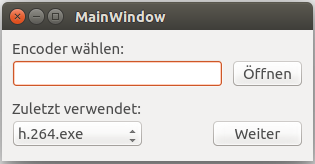
\includegraphics[width=0.4\textwidth]{GUI_Entwurf_1/GUI_1.png}
\caption{Encoderauswahl}
\end{figure}
\begin{itemize}
\item "Öffnen" öffnet einen "Datei öffnen Dialog"
\item Alternativ kann der Dateipfad manuell in das Textfenster eingegeben werden
\item "Zuletzt verwendet" bietet eine Auswahl der kürzlich verwendeten Encoder
\item "Weiter" bestätigt die Auswahl und wechselt zur Videoauswahl
\end{itemize}
\subsubsection{Videoauswahl}
\begin{figure}[htbp] 
\centering
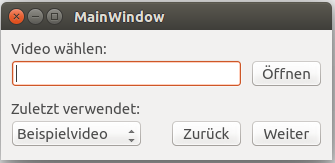
\includegraphics[width=0.5\textwidth]{GUI_Entwurf_1/GUI_2.png}
\caption{Videoauswahl}
\end{figure}
\begin{itemize}
\item "Öffnen" öffnet einen "Datei öffnen Dialog"
\item Alternativ kann der Dateipfad manuell in das Textfenster eingegeben werden
\item "Zuletzt verwendet" bietet eine Auswahl der kürzlich verwendeten Videos
\item "Weiter" bestätigt die Auswahl und wechselt zur Filter- und Musterauswahl
\item "Zurück" wechselt zur Encoderauswahl
\end{itemize}
\subsubsection{Filter/Artefakte}
\begin{figure}[htbp] 
\centering
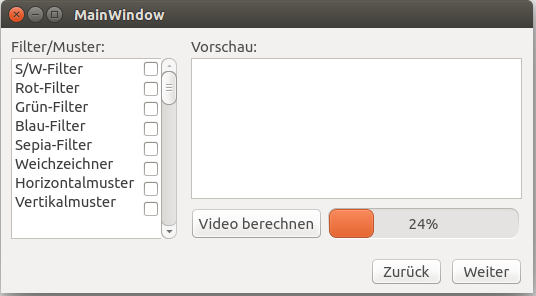
\includegraphics[width=0.5\textwidth]{GUI_Entwurf_1/GUI_3.png}
\caption{Filter/Artefakte Auswahl}
\end{figure}
\begin{itemize}
\item "Filter" bietet die Möglichkeit einen Filter auszuwählen
\item "Muster/Artefakte" bietet die Möglichkeit ein Muster oder ein Artefakt auszuwählen
\item "Vorschau" berechnet 5 Vorschau Frames
\item "<,>" bieten die Möglichkeit zwischen den Frames zu springen
\item "Video berechnen" wendet die ausgewählten Filter/Muster auf das gesamte Video an
\item "Play, Pause, Restart" bieten die Möglichkeit das berechnete Video abzuspielen
\item "Weiter" bestätigt die Auswahl und wechselt zur Wiedergabe und Auswertung
\item "Zurück" wechselt zur Videoauswahl
\end{itemize}
\subsubsection{Wiedergabe und Auswertung}
\begin{figure}[htbp]
\centering
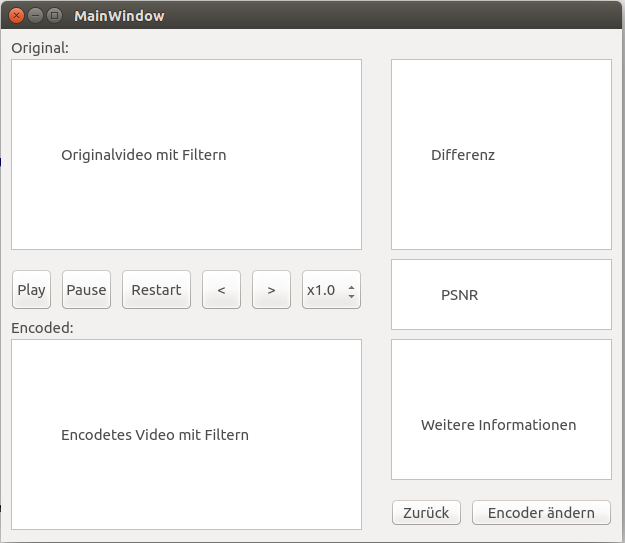
\includegraphics[width=0.5\textwidth]{GUI_Entwurf_1/GUI_4.png}
\caption{Wiedergabe und Auswertung}
\end{figure}
\begin{itemize}
\item "Play" Startet alle Videos
\item "Pause" Pausiert alle Videos
\item "Restart" Startet alle Videos neu
\item "<" Springt bei allen Videos einen Frame rückwärts
\item ">" Springt bei allen Videos einen Frame vorwärts
\item "x1.0" zeigt die aktuelle Wiedergabegeschwindigkeit und bietet die Möglichkeit diese zu ändern
\item "Differenz" zeigt Differenz oder Makroblöcke in dem Bereich oben rechts
\item "Weitere Informationen" kann Metadaten etc. enthalten
\item "Zurück" Wechselt zur Filter- und Musterauswahl
\item "Encoder ändern" öffnet einen "Datei öffnen Dialog" um den neuen Encoder zu wählen und wechselt dann zu Fenster 3 (alte Auswahl bleibt erhalten)
\end{itemize}
\section{Qualitätsbestimmungen}
\begin{tabular}{|c|c|c|c|c|}
\hline Robustheit & • &  &  & \\ 
\hline Zuverlässigkeit & • &  &  & \\ 
\hline Korrektheit & • &  &  & \\ 
\hline Benutzerfreundlichkeit & • &  &  & \\ 
\hline Effizienz &  & • &  & \\ 
\hline Portierbarkeit &  &  & • & \\ 
\hline Kompatibilität &  &  & • & \\ 
\hline Modifizierbarkeit &  &  & • & \\ 
\hline Sicherheit &  &  &  & • \\ 
\hline 
\end{tabular} 
\section{Globale Testfälle und Szenarien}
Folgende Funktionssequenzen sind zu überprüfen:
\subsection{Encoder auswählen}
\subsubsection{Encoder auswählen}
Programm starten, "Öffnen" klicken, im Dateisystem den Encoder auswählen
\subsubsection{Encoder aus Liste wählen}
Programm starten, unter "Zuletzt verwendet" einen Encoder wählen
\subsection{Video Auswählen}
\subsubsection{Video wählen}
Encoder wählen, "Öffnen" klicken, im Dateisystem das Video wählen
\subsubsection{Video aus Liste wählen}
Encoder wählen, unter "Zuletzt verwendet" ein Video wählen
\subsubsection{Filter auswählen}
Encoder und Video wählen, einzelne Filter ankreuzen
\subsubsection{Artefakte auswählen}
Encoder und Video wählen, einzelne Artefakte ankreuzen
\subsubsection{Vorschau anzeigen}
Encoder, Video, Filter und Artefakte wählen, "Vorschau drücken", "<", ">" verwenden
\subsubsection{Filter/Artefakte anwenden}
Encoder, Video, Filter und Artefakte wählen, "Video berechnen" drücken
\subsubsection{Vorschau des kompletten Videos}
Encoder, Video, Filter und Artefakte wählen, "Video berechnen" drücken, "Play", "Pause" und "Restart" Button verwenden
\subsection{Video encodieren}
Encoder, Video, Filter und Artefakte anwenden, "weiter" drücken
\subsection{Bewertung des Encoders}
\subsubsection{Anschauen des codierten und rohen Videos}
Encoder, video, Filter und Artefakte wählen, encodieren, unter rechte Seite der Gui betrachten
\subsubsection{Einstellen der Abspielgeschwindigkeit}
Encoder, video, Filter und Artefakte wählen, encodieren, "<", ">" und das Menü rechts von den beiden Buttons verwenden
\subsubsection{Bewertungskriterien anzeigen}
Encoder, video, Filter und Artefakte wählen, encodieren, untere rechte Seite der Gui betrachten
\subsubsection{Unterschied zwischen Roh- und encodiertem Video anzeigen}
Encoder, video, Filter und Artefakte wählen, encodieren, obere rechte Seite der Gui betrachten
\subsubsection{Interressante Eigenschaften des encodierten Videos anzeigen}
Encoder, video, Filter und Artefakte wählen, encodieren, im rechten, mittleren Menü jede Auswahl durchgehen
\end{document}